\documentclass[english]{article}

\usepackage[utf8]{inputenc}
\usepackage[english]{babel}
\usepackage{url}
\usepackage{listings}
\usepackage{amssymb}
\usepackage{todonotes}

\setcounter{secnumdepth}{-1}
\begin{document}
\newcommand{\Ci}{ \mathbb{C} }
\newcommand{\C}{ $\Ci$ }

\lstnewenvironment{bash}
{\lstset{language=bash, showstringspaces=false}}
{}

\lstnewenvironment{python}
{\lstset{language=python, showstringspaces=false}}
{}


\section{Assignment 4 (regex) (30 + 15 points/40 + 5 points)}
All solutions should be stored in a directory called \texttt{assignment5} in your private repository.
In this assignment, INF3331 students may solve the assignments for INF4331 to earn extra points.

\section{5.0: Background info on syntax highlighting (0 points)}
When you use a good editor to edit a file with Python code, it will color it to make it easier to read for humans. Generally speaking comments will have a color to make them stand out from the rest of the text, so it is easier for us to separate them from the ``active'' parts of the program.

\begin{center}
  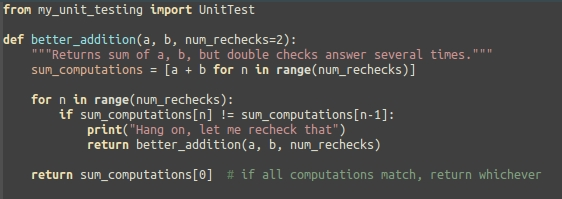
\includegraphics[height=3cm]{coloring_example.jpg}
\end{center}

In the first part of this assignment, you will create a program which does that, and make it extensible to use different color schemes and support different languages. It should read a regex dictionary from a file which in a sense specifies what parts of the language should be colored, and a color theme from another file which specifies what colors should be used.

For examples, take a look at the example files \texttt{naython.syntax}, \texttt{naython1.theme}, and \texttt{naython2.theme} which specifies the syntax of a very simple ``programming'' language and gives two different color themes to color it by. When your program is used to color \texttt{hello.ny}, your output should look like one of the two below, depending on which theme file you used:


\begin{center}
  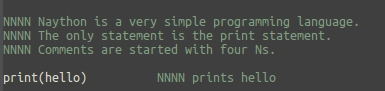
\includegraphics[width=7cm]{naython_colored_1}
  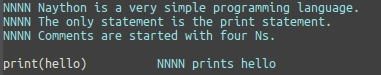
\includegraphics[width=7cm]{naython_colored_2}
\end{center}



\section{5.1: Syntax highlighting (7 points)}
Create a program which takes as input a regex , a color theme and a file and outputs the file with appropriate colors to standard out. Your program should be callable from the command line as \texttt{python3 highlighter.py syntaxfile themefile sourcefile\_to\_color} in the manner described above.

For more information on how to print in color, see clarifications.

Name of file: \texttt{highlighter.py}.


\section{5.2: Python syntax \\ (INF3331: 10 points + 5 bonus points) (INF4331: 15 points)}
Create a regex dictionary and color theme for Python. Your files should be usable by your program and follow the format specified in 5.0 - look at the naython examples for guidance. Choose at least 7 (INF4331: at least 10. INF3331: For bonus points, choose at least 10.) pieces of Python syntax from the below list and include them in your dictionary. Then create a second color theme. The color themes should be different, but you are free to use whichever colors you think look nicest.


\begin{itemize}
\item Comments
\item Function definitions
\item Class definitions
\item Strings
\item Imports
\item ``Special'' statements \texttt{None, True, False}
\item Variable assignments
\item Decorators
\item Try/except
\item for-loops
\item while-loops
\item if/elif/else blocks
\item Something else you feel is missing (be reasonable)

\end{itemize}

Name of files: \texttt{python.syntax}, \texttt{python.theme},  \texttt{python2.theme}

\section{5.3: Syntax for your favorite language (INF3331: 5 bonus points, INF4331: 5 points)}
Create a regex dictionary and color theme for your favorite language. See clarifications for requirements.

Name of files: \texttt{favorite\_language.syntax}, \texttt{favorite\_language.theme}

\section{5.4: Syntax for your second favorite language (INF3331 and INF4331, up to 5 bonus points)}
For 5 bonus points, repeat 5.3 for a different language. See clarifications for requirements.

Name of files: \texttt{favorite\_language.syntax}, \texttt{favorite\_language.theme}



\section{5.5: superdiff (10 points)}
 % \todo{It's hard to describe what specifically should be output without also telling them what algorithm to use, and I think it might be a nice experience for them to have a not-entirely-well-constrained problem. Thoughts?}
The standard utility \texttt{diff} takes two files as input, and outputs a file containing all changes which have to be made to the first file to make it into the second file. In this assignment, you will create your own implementation of the standard \texttt{diff} utility. For convenience, your implementation should take two filenames from the command line, and treat the first as the ``original'' version of a file, and the second as a modified version.

It should then go through the files line by line, and if a line has not been modified, print it with a \texttt{0} in front, if it has been added, print it with a \texttt{+} in front, and if it has been deleted, print it with a \texttt{-} in front. If a line has been modified, treat it as being a deletion of the original line, and then an addition of the modified line.

Name of file: \texttt{my\_diff.py}


\section{5.6: Coloring diff (3 points)}
In this assignment, you will take the output from \texttt{my\_diff.py} and color it so that additions become green, deletions become red and no-change lines aren't colored in any special way. As you might notice, this is similar to what you did before, so instead of making a new script, make your program as a syntax file and color theme for your syntax highlighter.

Name of files: \texttt{diff.syntax}, \texttt{diff.theme}



\newpage

\section{Clarifications}

\subsection{5.0 (general clarifications)}
\begin{itemize}
\item Your \texttt{.syntax} files should have lines of the form \texttt{regex: name} where regex is a quoted string specifying a regex, and name is some arbitrary alphabetical string giving some name to the thing specified by the regex. See \texttt{naython.syntax} for an example.
\item Your \texttt{.theme} files should have lines of the form \texttt{name: color\_sequence} where \texttt{name} is one of the names specified in the matching \texttt{.syntax} file, and \texttt{color\_sequence} is some bash color sequence. (i.e. something which would be valid if you did \texttt{"\textbackslash033[\{\}m".format(color\_sequence)}
\end{itemize}


\subsection{5.1}
\begin{itemize}
\item Information on printing in color can be found in \url{http://misc.flogisoft.com/bash/tip_colors_and_formatting}, and an example in \texttt{coloring\_example.py} in the student resources repository.

Note that you need to be careful with printing in color when two regexes ``overlap''. For example, if you for example have decided to color Python strings blue and newline characters green, coloring \texttt{``Line 1 \textbackslash n Line 2''} properly means printing first the color sequence for blue, then \texttt{``Line 1 }, then the color sequence for green, then \texttt{\textbackslash n}, then the color sequence for blue, then \texttt{ Line 2''}. So your program needs to ``notice'' that it needs to re-insert the blue color sequence in the middle of the string.
\end{itemize}


% \subsection{5.2}
% Nothing yet!

% \subsection{5.3}
% Nothing yet!



\subsection{5.3, 5.4}
\begin{itemize}

\item Use your best judgment on how much work you should expect to do here. If you make a complete syntax highlighter for whitespace, that is very cute, but you should not expect to get 5 points. On the other hand, if you manage to color a decent (but not all) subset of Java, that is probably enough. 
\item Make sure to choose ``sufficiently different'' languages in 5.2, 5.3 and 5.4. In particular, even though your favorite language might be Python 2, don't expect to get 10 points for doing Python 3 in 5.2, and then 5 more for doing it in 5.3 or 5.4. :) If you are unsure about this point, feel free to ask on Piazza.

\end{itemize}

\subsection{5.5}
\begin{itemize}
\item There is some ambiguity inherent to the problem. For example, if the original has the lines ``A'', ``B'' and the modified version has the lines ``B'', ``A'', was ``A'' deleted and later inserted, or was ``B'' inserted and later deleted? There are a lot of strange edge cases, so don't be too worried about making an implementation which handles absolutely all of them.
\item Try to make sure that your program is ``reasonable'' (i.e. if the original is ``A'', ``B'', ``C'', ``D'', ``E'', ``F'' and the modified file is ``B'', ``C'', ``D'', ``E'', ``F'', ``G'', your program should ideally output that ``A'' has been deleted and ``G'' has been inserted at the end, and not say ``everything in the first file was deleted, then everything in the second file was inserted''.
\end{itemize}

\subsection{5.6}
\begin{itemize}
\item Your syntax and theme should work so that if the output from \texttt{my\_diff.py} (5.6) is stored in the file \texttt{diff\_output.txt}, the call \texttt{python3 highlighter.py diff.syntax diff.theme diff\_output.txt} should produce the desired colored diff.
\end{itemize}





\end{document}


